\section{Analytic equilibrium for the polytropic disk}\label{appen1}
For a polytropic disk with $P = K\rho^2$ the dimensional equilibrium equation to
be solved is 
\begin{align}
  0=\csmid^2\frac{d^2}{dz^2}\left(\frac{\rho}{\rho_0}\right) +
  \Omega_z^2 + \frac{\Omega^2}{Q}\left(\frac{\rho}{\rho_0}\right), 
\end{align}
which is obtained by combining Eq. \ref{eqm_eqns1} and
\ref{eqm_eqns2} with the above equation of state. The solution is
\begin{align}  
  \frac{\rho}{\rho_0} = \left(1 + \frac{\Omega_z^2}{\Omega^2}Q\right)\cos{\left(a z\right)} - 
  \frac{\Omega_z^2}{\Omega^2}Q,  
\end{align}
where  
\begin{align}
  a^2 \equiv \frac{\Omega^2}{Q\csmid^2}. 
\end{align}
The polytropic disk thickness is
\begin{align}
  H =
  \frac{\csmid}{\Omega}\sqrt{Q}\arccos\left(\frac{\Omega_z^2Q}{\Omega^2+ \Omega_z^2Q}\right).  
\end{align}
Given a fixed mid-plane temperature, the function $f(Q)\equiv
\csmid/\Omega H$ is an inverse measure of the disk thickness, and $f$ increases with decreasing $Q$,
as shown in Fig. \ref{plot_fq}. This corresponds to a thinner disk
with increasing strength of vertical self-gravity.

\begin{figure}
  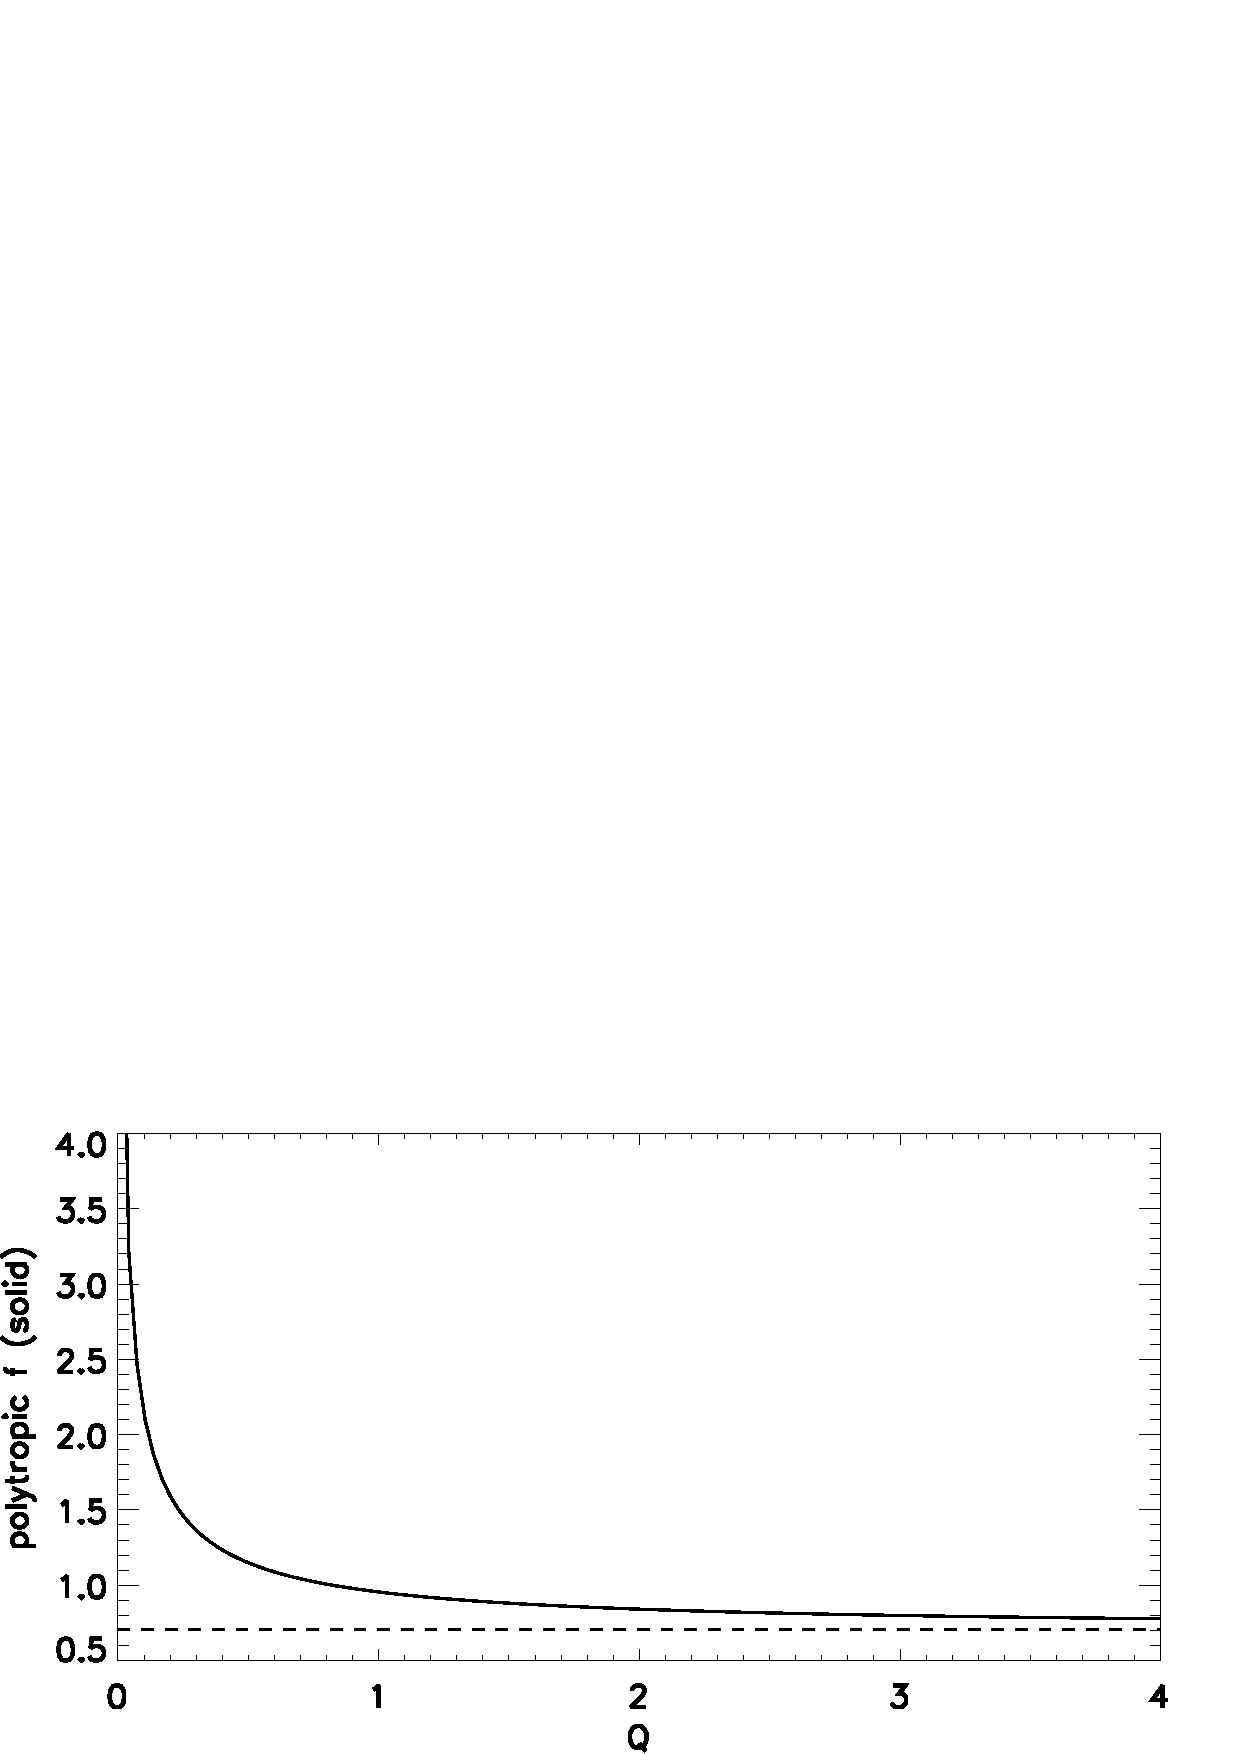
\includegraphics[width=\linewidth]{figures/plot_fq}
  \caption{The function $f(Q)$ describing vertical hydrodstatic 
    equilibrium in self-gravitating polytropic disks (solid line). The
    horizontal dashed line is the asymptotic value of $1/\sqrt{2}$ for
    large $Q$.  
    \label{plot_fq}}
\end{figure}

\section{Relation between $Q$ and the Toomre parameter}\label{q3d2d}
The Toomre parameter defined for razor-thin disks is 
\begin{align} 
  Q_\mathrm{2D}\equiv \frac{\kappa c_s}{\pi G\Sigma},  
\end{align}
where $\Sigma$ is the total column density. To relate our
self-gravity parameter $Q$ and $Q_\mathrm{2D}$, we replace $c_s$ by
$\overline{c_s}\equiv\int\rho c_s dz/\int\rho dz$, and 
$\kappa$ by $\Omega$, giving
\begin{align}
  Q_\mathrm{2D} = 2Qf \frac{\int_0^1
    \hat{\rho} \hat{c}_s
    d\hat{z}}{\left(\int_0^1 \hat{\rho} d\hat{z}\right)^2},   
\end{align}
where each term on the right-hand-side is non-dimensionalized (see
\S\ref{non-dim}). Fig. \ref{plot_q3d2d} plots this relation 
for isothermal and polytropic disks.  

\begin{figure}
  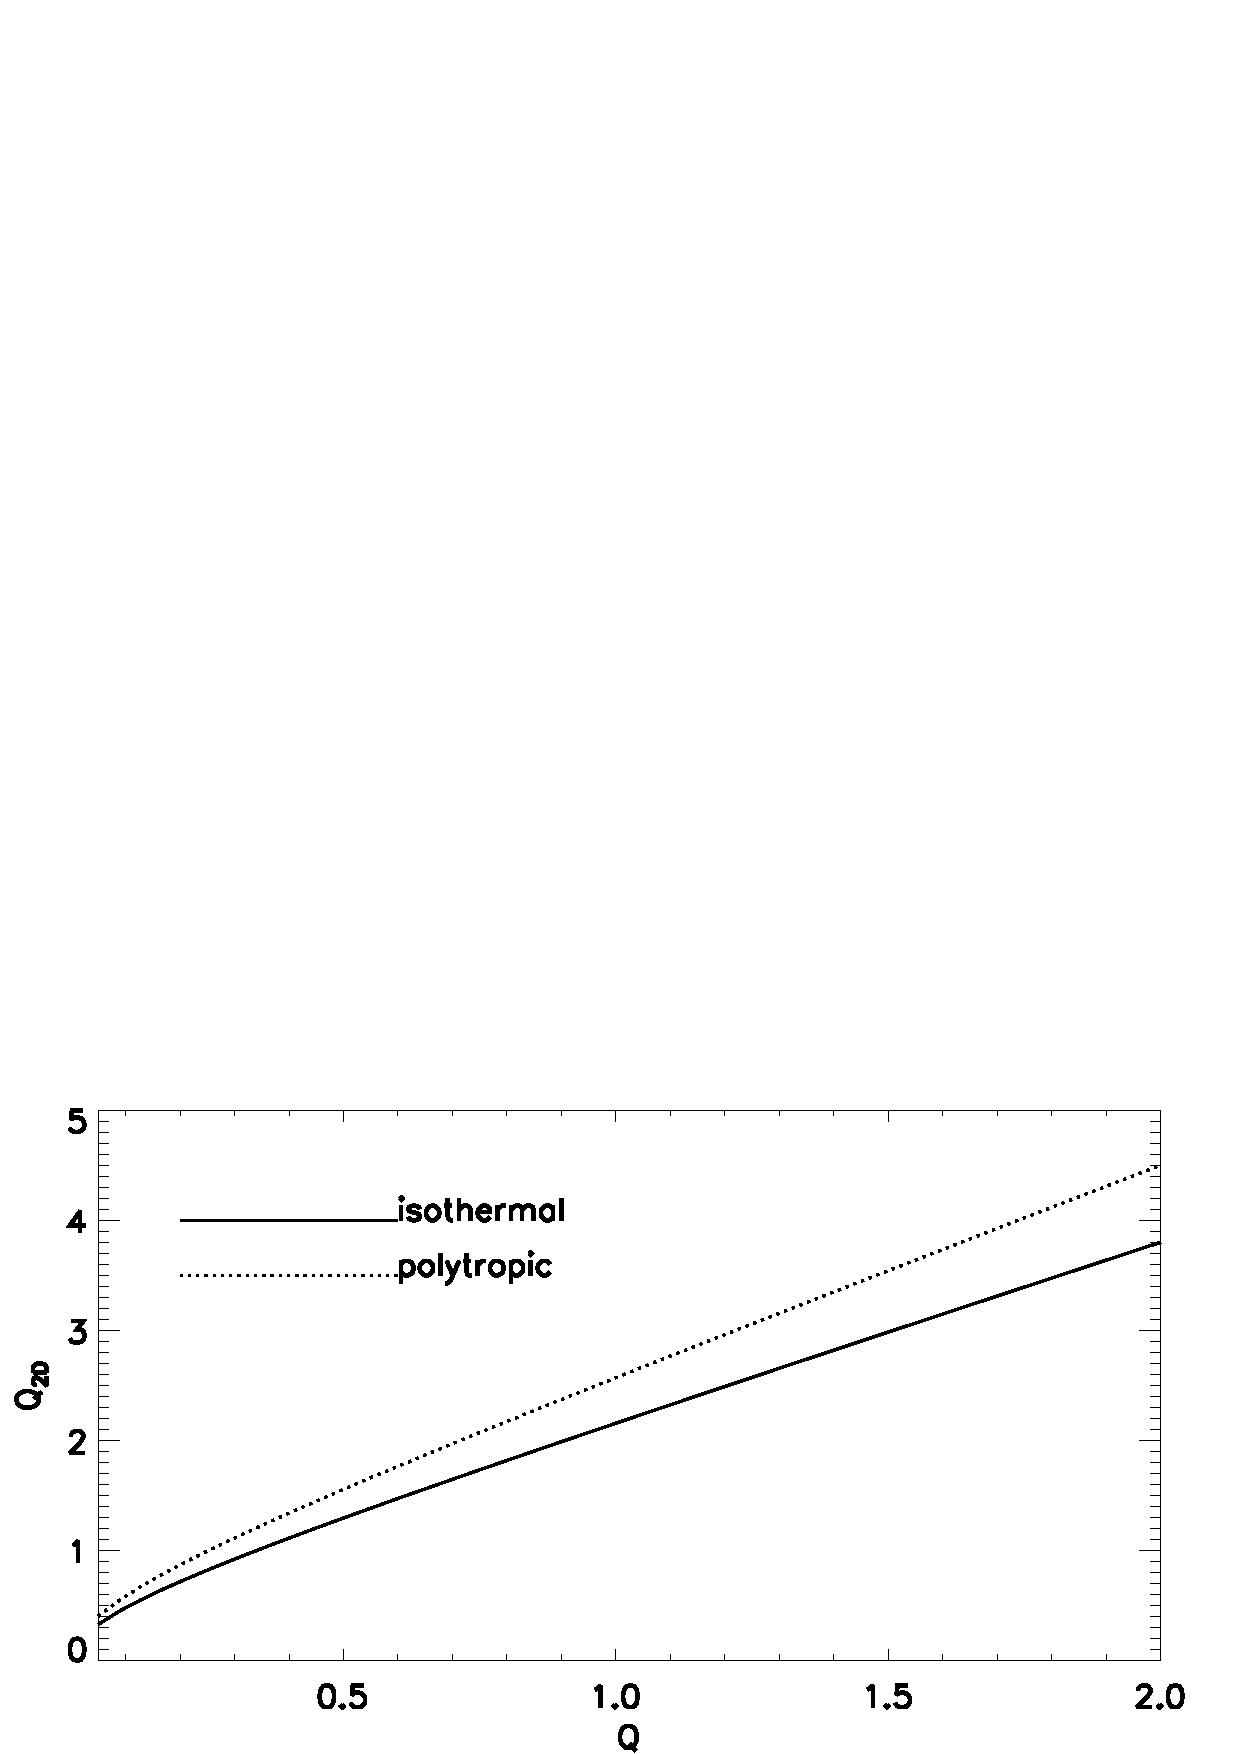
\includegraphics[width=\linewidth]{figures/q2d_iso}
  \caption{Relation between the self-gravity parameter $Q$ used in
    this paper and the Toomre parameter $Q_\mathrm{2D}$ for razor-thin
    disks. 
    \label{plot_q3d2d}}
\end{figure}


\section{Reduction to linear hydrodynamics}\label{reduction} 
Our task here is to remove the magnetic field and vertical velocity
perturbations from the linearized equations. Let us first define operators
\begin{align}
  D_0 = 1, \quad D_1 = \frac{\rho^\prime}{\rho} + \frac{d}{dz}, \quad
  D_2 = \frac{\rho^{\prime\prime}}{\rho} +
  \frac{2\rho^\prime}{\rho}\frac{d}{dz} + \frac{d^2}{d z^2},
\end{align}
and 
\begin{align}
  \overline{D}_0 = \eta D_0, \quad \overline{D}_1 = \eta^\prime D_0 + \eta
  D_1,\quad \overline{D}_2 = \eta^{\prime\prime} D_0 + 2\eta^\prime D_1 +
  \eta D_2. 
\end{align}
And we define the variables
\begin{align}
  &U \equiv \imgi\sigma\dvx - 2\Omega\dvy + \imgi k_x \w,\\
  &V \equiv \imgi\sigma\dvy + \frac{\kappa^2}{2\Omega}\dvx.
\end{align}

We first express the continuity equation in terms of horizontal
velocity, density and potential perturbations. 
The vertical velocity perturbation is 
\begin{align}
  \dvz = \frac{\imgi}{\sigma}\left(\w^\prime + \epsilon V\right),  
\end{align}
where the linearized $y$ momentum equation was used (i.e. eliminating
$\dby^\prime$ between Eq. \ref{lin_vy} and Eq. \ref{lin_vz}). 
Inserting this into the linearized continuity equation
(Eq. \ref{lin_cont}), we obtain
\begin{align}
0 = W^{\prime\prime} + \left(\ln{\rho}\right)^\prime W^\prime +
\frac{\sigma^2}{c_s^2}W +  \dphi^{\prime\prime} + \left(\ln{\rho}\right)^\prime \dphi^\prime
 + \sigma k_x \dvx + \epsilon D_1 V.
%  0=  W^{\prime\prime} + \left(\ln{\rho}\right)^\prime W^\prime +
%  \frac{1}{c_s^2f^2}\left(\frac{\rho}{Q} + \sigma^2\right)W +
% \left(\ln{\rho}\right)^\prime\dphi^\prime + k_x^2\dphi + \frac{\sigma
%    k_x}{f}\dvx.\label{final_w}
\end{align}

Next, we examine separately the cases of a vertical field with
variable resistivity and that of a tilted field with uniform
resistivity. (A similar procedure can be performed in
the general case of a tilted field with variable resistivity.) 

\subsection{Vertical field with variable resistivity}
First consider $\epsilon = 0$ and $\eta=\eta(z)$ in the linearized
equations. Denoting the $n^\mathrm{th}$ vertical derivative as $^{(n)}$, the
equations of motion give
\begin{align}
  &\dbx^{(n)} = \frac{\mu_0\rho}{B_z}D_{n-1}U + \imgi k_x \dbz^{(n-1)},\label{bx_eq}\\
  &\dby^{(n)} = \frac{\mu_0\rho}{B_z}D_{n-1}V,\label{by_eq}
\end{align}
for $n\geq1$. Differentiating the divergence-free condition for the magnetic
field gives
\begin{align}
  \imgi k_x \dbx^{\prime} + \dbz^{\prime\prime} = 0.   
\end{align}
We insert the expression for $\dbx^\prime$ from Eq. \ref{bx_eq} and the
expression for $\dbz^{\prime\prime}$ from the $z$ component of the
linearized induction equation (Eq. \ref{induct_vert}) to obtain
\begin{align}\label{bz_eq}
  -\sigma\dbz^{(n)} = k_x B_z \dvx^{(n)} + k_x\frac{\mu_0\rho}{B_z}\overline{D}_nU. 
\end{align}

%\subsection{Eliminating $\dbx$}
Inserting the above expressions for $\dbx^{\prime\prime}$,
$\dbx^\prime$ (Eq. \ref{bx_eq}) and $\dbz^\prime$  (Eq. \ref{bz_eq})
into the right-hand-side of the $x$-induction equation (Eq. \ref{induct_x} ) gives   
\begin{align}
  \imgi\sigma \dbx =
  B_z\dvx^\prime + \frac{\mu_0\rho}{B_z}\overline{D}_1U. \label{bx_expression}
\end{align}
($\bar{\sigma}\neq0$ has been assumed to obtain this.) We
differentiate this expression with respect to $z$ and eliminate the
resulting $\dbx^\prime$ using Eq. \ref{bx_eq}, to obtain
\begin{align}
%  0 = B_z\dvx^{\prime\prime} -
%  k_x^2B_z\dvx + \frac{\mu_0\rho}{B_z}\left(\overline{D}_2 - k_x^2 \overline{D}_0
%    - \imgi\sigma D_0\right)U. \label{final_vx} 
  0 = v_A^2\left(\dvx^{\prime\prime} -
  k_x^2\dvx\right) + \left(\overline{D}_2 - k_x^2 \overline{D}_0
    - \imgi\sigma D_0\right)U. \label{final_vx} 
\end{align}

%\subsection{Eliminating $\dby$}
We follow a similar procedure as above to remove $\dby$. 
We use Eq. \ref{bx_expression} and Eq. \ref{by_eq} to 
eliminate $\dbx,\dby^\prime$ and $\dby^{\prime\prime}$ from the
right-hand-side of the $y$-induction equation (Eq. \ref{induct_y}), 
%\begin{align}
%  &\imgi\bar{\sigma}\dby = f\dvy^\prime - \imgi
%  S\frac{\dbz^\prime}{k_x} +
%  \eta\dby^{\prime\prime}+\eta^\prime\dby^\prime.  
%\end{align}
%We can now insert expressions for the magnetic field derivatives using
%Eq. \ref{by_eq} and \ref{bz_eq} to obtain an expression for $\dby$, 
\begin{align}
  \imgi\bar{\sigma}\dby = B_z\dvy^\prime + \frac{\imgi S}{\sigma}\left(
    B_z\dvx^\prime + \frac{\mu_0\rho}{B_z}\overline{D}_1U\right) +
  \frac{\mu_0\rho}{B_z}\overline{D}_1V. \label{by_expression}
\end{align}
We differentiate this expression with respect to $z$, then eliminate 
$\dby$ and  $\dby^\prime$ from the left-hand-side of the resulting
expression using Eq. \ref{by_expression} and 
Eq. \ref{by_eq}, respectively. We obtain
\begin{align}
0 = v_A^2\left(\dvy^{\prime\prime} -
\frac{\sbar^\prime}{\sbar}\dvy^\prime\right)  
+ \frac{\imgi S v_A^2}{\sigma}\left(\dvx^{\prime\prime} -
\frac{\sbar^\prime}{\sbar}\dvx^\prime\right) + \frac{\imgi
  S}{\sigma}\left(\overline{D}_2 -
    \frac{\sbar^\prime}{\sbar}\overline{D}_1 \right)U 
+\left(\overline{D}_2 -
    \frac{\sbar^\prime}{\sbar}\overline{D}_1 - \imgi\sbar D_0 \right)V. \label{final_vy}
%0 = B_z\left(\dvy^{\prime\prime} -
%\frac{\sbar^\prime}{\sbar}\dvy^\prime\right)  
%+ \frac{\imgi S B_z}{\sigma}\left(\dvx^{\prime\prime} -
%\frac{\sbar^\prime}{\sbar}\dvx^\prime\right) + \frac{\imgi
%  S}{\sigma}\frac{\mu_0\rho}{B_z} \left(\overline{D}_2 -
%    \frac{\sbar^\prime}{\sbar}\overline{D}_1 \right)U 
%+\frac{\mu_0\rho}{B_z} \left(\overline{D}_2 -
%    \frac{\sbar^\prime}{\sbar}\overline{D}_1 - \imgi\sbar D_0 \right)V. \label{final_vy}
%
%  0 =& \frac{f^2}{\beta\rho}\left(\dvy^{\prime\prime} -
%  \frac{\bar{\sigma}^\prime}{\bar{\sigma}}\dvy^\prime\right) 
%  + \sbar\sigma D_0\dvy  + \frac{\imgi 
%    S}{\sigma}\frac{f^2}{\beta\rho}\left(\dvx^{\prime\prime} -
%    \frac{\sbar^\prime}{\sbar}\dvx^\prime\right) -
%    \frac{\imgi\sbar\kappa^2}{2}D_0\dvx \notag\\
%    & + \left(\overline{D}_2 -
%    \frac{\sbar^\prime}{\sbar}\overline{D}_1\right)\left[\imgi\left(\sigma
%      - \frac{2S}{\sigma}\right)\dvy + \left(\frac{\kappa^2}{2} -
%      S\right)\dvx - \frac{Sfk_x}{\sigma}\w\right]. \label{final_vy}
\end{align}

Eq. \ref{final_vx} and \ref{final_vy} constitutes the first two
linearized equations to be solved.

\subsection{Tilted field with uniform resistivity}
Here we allow $\epsilon\neq 0$ but take $\eta$ to be constant. We
first obtain expressions for $\dbx$ and $\dby$. Differentiating
the $x$ momentum equation and replacing the resuting $\dbz^\prime$
using the divergence-free condition and $\dby^\prime$ using the $y$
momentum equation, we obtain an expression for $\dbx^{\prime\prime}$
which can be inserted into the $x$ induction equation. This gives
\begin{align}
  \imgi\sigma\dbx = B_z\dvx^\prime +
  \frac{\eta\mu_0\rho}{B_z}\left( D_1 U + \imgi\epsilon k_x D_0
  V\right).\label{bx_tilted}  
\end{align}
We can insert this into the $y$ induction equation to obtain
\begin{align}
  \imgi\sbar\dby = -B_y\Delta + B_z\dvy^\prime + \frac{\imgi
    S}{\sigma}\left[ B_z \dvx^\prime+ \frac{\eta\mu_0\rho}{B_z}\left( D_1 U + \imgi\epsilon k_x D_0
  V\right)\right] + \frac{\eta\mu_0\rho}{B_z}D_1V,\label{by_tilted}
\end{align} 
where we have also used the derivative of the $y$ momentum equation to
eliminate  $\dby^{\prime\prime}$. Recall $\Delta \equiv i k_x \dvx +
\dvz^\prime$, so that
\begin{align}
  \Delta = \imgi k_x \dvx + \frac{i}{\sigma}\left(\w^{\prime\prime} +
  \epsilon V^\prime\right) = -\left[\frac{\imgi\sigma W}{c_s^2} +
    \frac{\imgi\left(\ln{\rho}\right)^\prime}{\sigma}\left(\w^\prime +
    \epsilon V\right)\right], 
\end{align}
where the second equality results from the continuity equation. 

Now consider
\begin{align}
  \dbx^\prime - \imgi k_x \dbz = \frac{\mu_0\rho}{B_z}D_0U +
  \imgi\epsilon k_x \dby = \frac{\sigma}{\sbar}\dbx^\prime +
  \frac{\imgi k_x^2B_z}{\sbar}\dvx,
\end{align}
where the first equality corresponds to the $x$ momentum equation and
the second equality results from replacing $\dbz$ using the $z$
induction equation. We can now use the above expressions for $\dbx$
and $\dby$ (Eq. \ref{bx_tilted}--\ref{by_tilted}) to obtain
\begin{align}
0 = &v_A^2\left[k_x^2\left(1+\epsilon^2\right)\dvx - \frac{\epsilon k_x
  S}{\sigma}\dvx^\prime - \dvx^{\prime\prime}\right] + \imgi\epsilon
k_x v_A^2 \dvy^\prime + \frac{\epsilon^2 k_x
  v_A^2}{\sigma}\left(\w^{\prime\prime} + \epsilon V^\prime\right) 
\notag\\ &-\left[\eta\left(D_2 + \frac{\epsilon k_x S}{\sigma}D_1\right) -
  \imgi\sbar D_0 \right]U %\notag\\
- \frac{\imgi\epsilon^2k_x^2S}{\sigma}\eta D_0V.
\end{align}
%We can now use the above expression for $\dbx,\dby$ to eliminate
%$\dbx^\prime$ and $\$ in the $x$ momentum equation  
%\begin{align}
%  \dbx^\prime - \imgi k_x\dbz = \frac{}{}
%\end{align}

Similarly, we differentiate Eq. \ref{by_tilted} and use the $y$
momentum equation to eliminate $\dby^\prime$ to obtain
\begin{align}
0 = &v_A^2\dvy^{\prime\prime} + \frac{\imgi S}{\sigma}v_A^2
\dvx^{\prime\prime} +\frac{\imgi S}{\sigma}\eta D_2U +
\left\{\eta\left(D_2 - \frac{\epsilon k_x S}{\sigma} D_1\right) +
  \imgi\left[\frac{\epsilon^2v_A^2\left(\ln{\rho}\right)^{\prime\prime}}{\sigma}
    - \sbar\right]D_0\right\}V \notag\\ &+ \imgi\epsilon
  v_A^2\left\{\frac{\sigma}{c_s^2}\left[W^\prime -
    \left(\ln{c_s^2}\right)^\prime W\right] +
    \frac{1}{\sigma}\left[\left(\ln{\rho}\right)^\prime(\w^{\prime\prime}
      + \epsilon V^\prime)
      +\left(\ln{\rho}\right)^{\prime\prime}\w^{\prime} \right]\right\}.    
\end{align}

%\subsection{Non-dimensionalization}
%In practice we solve the linearized equations in non-dimensional form,
%by defining
%We further write 
%\begin{align}
%  &z=\hat{z}H,\quad k_x =  \hat{k}_x/H,\quad \sigma = \hat{\sigma}\Omega,
%  \quad \delta\bm{v} = \csmid 
%  \delta\hat{\bm{v}}, \\ 
%  &\delta\bm{B} = B\delta\hat{\bm{B}},\quad
%  \delta\rho = \rho\hat{W}/\hat{c}_s^2,\quad \delta\Phi =
%  \csmid^2\delta\hat{\Phi}, 
%\end{align}
%where we have introduced the non-dimensional enthalpy perturbation
%$\hat{W}$ and the sound-speed $\hat{c}_s=\csmid^{-1}\sqrt{dP/d\rho}$ can be 
%obtained from the equation of state. The background frequencies are
%written $S=\hat{S}\Omega$ and $\Omega_z=\hat{\Omega}_z\Omega$ and the 
%resistivity as $\eta = \hat{\eta}H^2\Omega$. 

%We will now drop the $\hat{\phantom{a}}$ notation. Henceforth it is
%understood that all variables have been appropriately normalized
%(i.e. $\Omega\to 1$ and $H\to 1$), unless otherwise stated.


%tilted field
% calculate b field vertical derivatives carefully
% try no velocity pert at bc
% try anti-aligned field 
